\documentclass[12pt]{beamer}
%\documentclass[20pt,handout]{beamer}
\usetheme{Darmstadt}
\usepackage{graphicx}
%\usepackage[german]{babel}
%\usepackage{ngerman}
\usepackage[T1]{fontenc}
\usepackage[utf8]{inputenc}
\usepackage{tikz}
\setbeamertemplate{footline}[frame number]

\newcommand{\cc}[1]{\includegraphics[height=4mm]{img/#1.png}\hspace{1mm}}
\usepackage{ifthen}
\newcommand{\license}[2][]{\\#2\ifthenelse{\equal{#1}{}}{}{\\\scriptsize\url{#1}}}
\usepackage{textcomp}
\usepackage{hyperref}

\pgfdeclareimage[height=.6cm]{c3d2logo}{./img/c3d2.pdf}


\pgfdeclarelayer{foreground}
\pgfsetlayers{main,foreground}
\logo{\pgfputat{\pgfxy(-1,0)}{\pgfbox[center,base]{\pgfuseimage{c3d2logo}}}}


\title{Unsere Datenspuren im Netz}
\author{Stephan Thamm\\\large Chaos Computer Club Dresden}
\date{19.06.2015}

\begin{document}
\maketitle

\section{Einleitung}
\subsection{}

\begin{frame}
  \frametitle{Chaos Computer Club}
  \begin{figure}
    \includegraphics<1>[height=0.7\textheight]{img/trojaner.png}
    \includegraphics<2>[height=0.7\textheight]{img/pentabug.jpg}
  \end{figure}
\end{frame}

\begin{frame}
    \frametitle{Chaos Computer Club Dresden}
    \begin{center}
	
\includegraphics[height=0.1\textheight]{img/c3d2_logo.png}
    \end{center}
    \begin{itemize}
      \item<1-> Chaos Computer Club Dresden (\url{https://c3d2.de})          
      \item<2-> Datenspuren: 24. und 25. Oktober 2015 (\url{https://datenspuren.de})
      \item<3-> Podcasts (\url{https://c3d2.de/radio.html})
      \item<4-> Chaos macht Schule (\url{https://c3d2.de/schule.html})
    \end{itemize}
\end{frame}

\begin{frame}
    \frametitle{Stasi vs. NSA}
    \only<1>{
      \begin{center}
        "Wir wissen z.B., dass es nicht so ist, wie bei der Stasi und dem KGB, dass es dicke Aktenbände gibt, wo unsere Gesprächsinhalte alle aufgeschrieben und schön abgeheftet sind. Das ist es nicht."
        \end{center}
        \hfill \tiny Bundespräsident Gauck zur NSA-Überwachung
    }
    \includegraphics<2>[height=0.7\textheight]{img/akten1.png}
    \includegraphics<3>[height=0.7\textheight]{img/akten2.png}
\end{frame}


\section{Daten sammeln}
\subsection{}

\begin{frame}
    \frametitle{Tempora}
    \begin{center}
      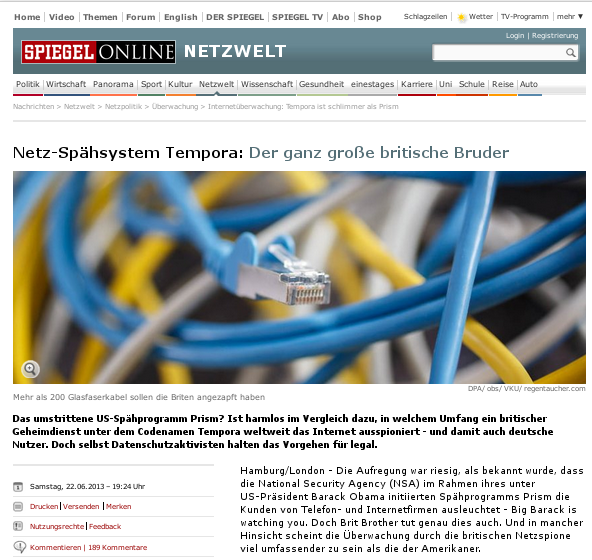
\includegraphics[height=0.7\textheight]{img/spiegel-tempora.png}
    \end{center}
\end{frame}

\begin{frame}
    \frametitle{Internet}
    \pause
    \begin{center}
      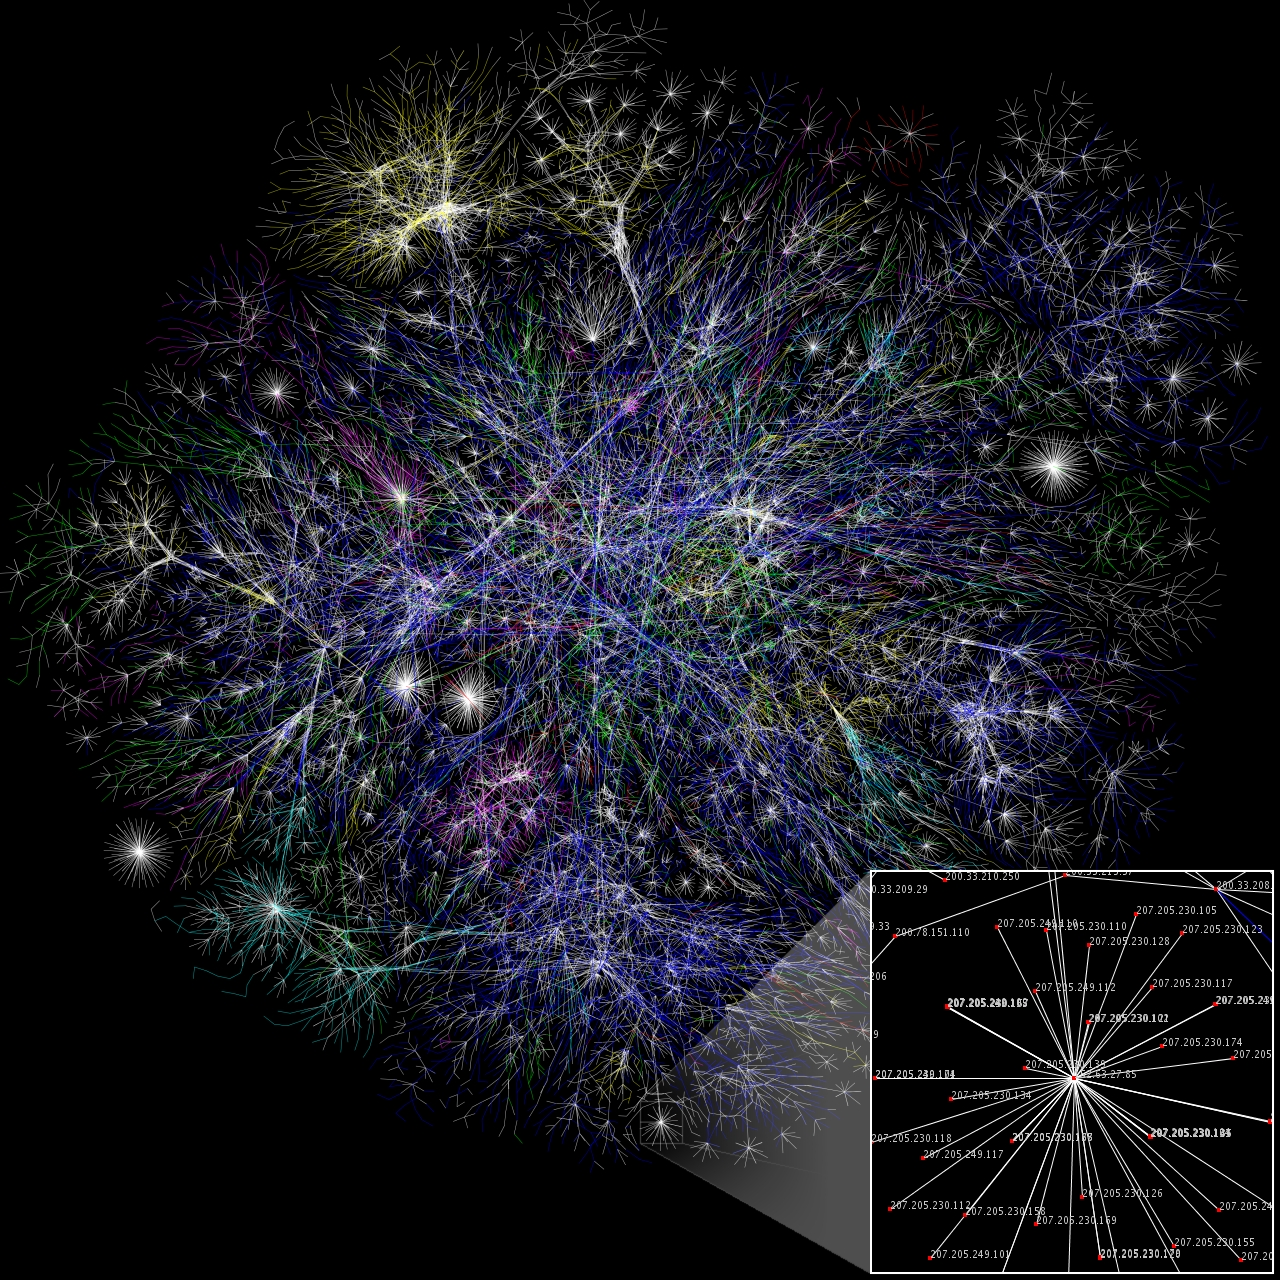
\includegraphics[height=0.7\textheight]{img/Internet_map_1024.jpg}
      {\\ \tiny \href{http://commons.wikimedia.org/wiki/File:Internet_map_1024.jpg}{Grafik}: \href{http://creativecommons.org/licenses/by/2.5/deed.en}{\cc{by}} The Opte Project}
    \end{center}
\end{frame}

\begin{frame}
    \frametitle{Prism}
    \begin{center}
      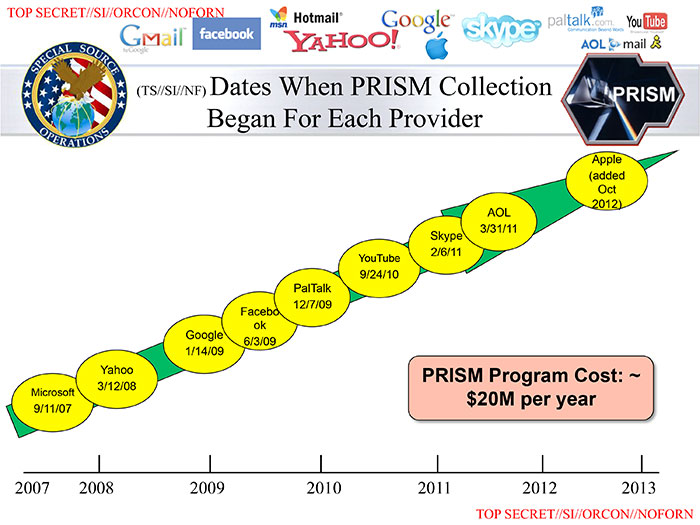
\includegraphics[height=0.7\textheight]{img/prism.jpg}
    \end{center}
\end{frame}

\begin{frame}
    \frametitle{Geschäftsmodelle}
    \pause
    \begin{figure}
      
\includegraphics[height=0.6\textheight]{img/business_pigs.jpg}
      \license[http://geekandpoke.typepad.com/geekandpoke/2010/12/the-free-model.html]{\cc{by-sa}}
    \end{figure}
\end{frame}

\begin{frame}
    \frametitle{Wert von Daten}
    \pause
    \begin{center}
      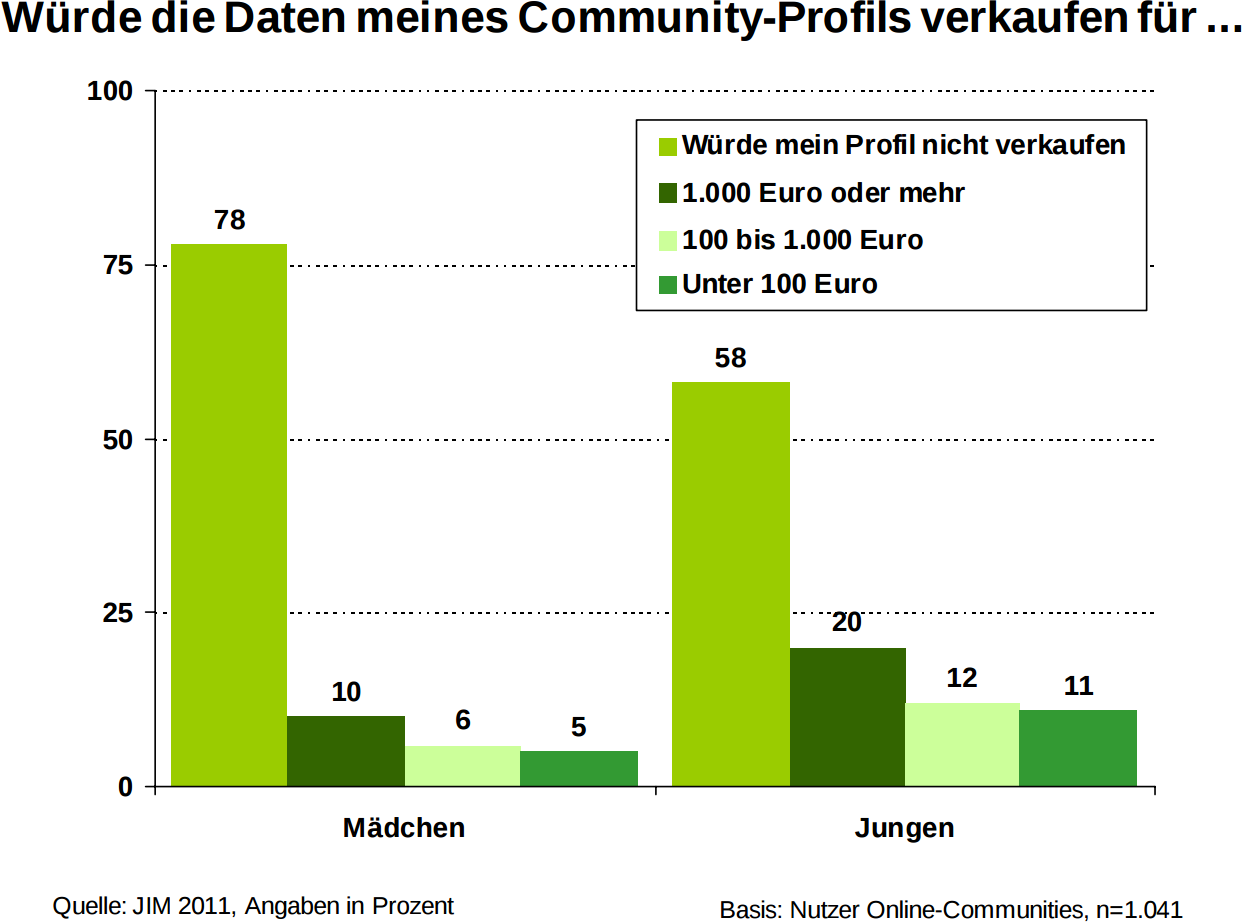
\includegraphics[width=0.7\textwidth]{img/daten.png}
    \end{center}
\end{frame}

\begin{frame}
    \frametitle{Lightbeam}
    \begin{center} 
        \includegraphics<1>[width=0.5\textwidth]{img/lightbeam.png}
        \includegraphics<2>[width=0.7\textwidth]{img/lightbeam_1.png}
        \includegraphics<3>[width=0.7\textwidth]{img/lightbeam_2.png}
    \end{center}
\end{frame}


\section{Daten auswerten}
\subsection{}

\begin{frame}
    \frametitle{Vorratsdaten}
    \pause
    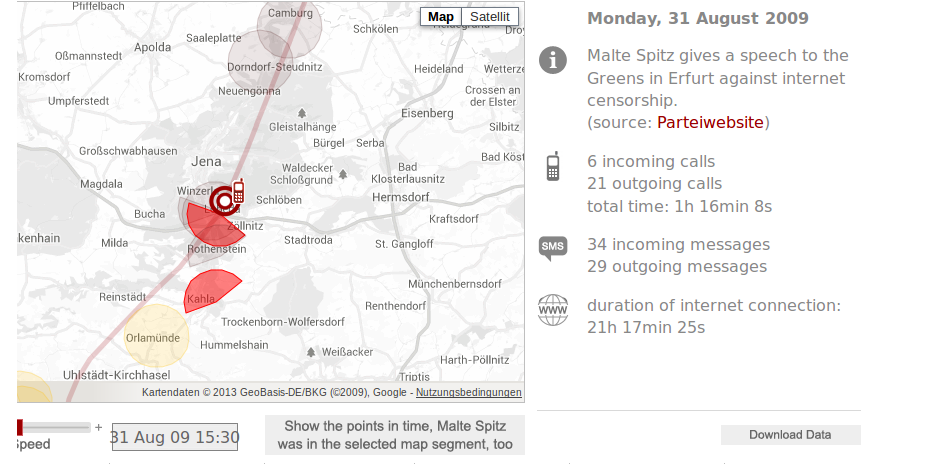
\includegraphics[height=0.7\textheight]{img/maltespitz.png}
\end{frame}

\begin{frame}
    \frametitle{Google Takeout}
    \pause
    \begin{center}
      \includegraphics[width=0.8\textwidth]<2>{img/google_heat_1.png}
      \includegraphics[width=0.8\textwidth]<3>{img/google_heat_2.png}
    \end{center}
\end{frame}

\begin{frame}
    \frametitle{Zeitstempel}
    \pause
    \begin{center}
      \only<2>{
        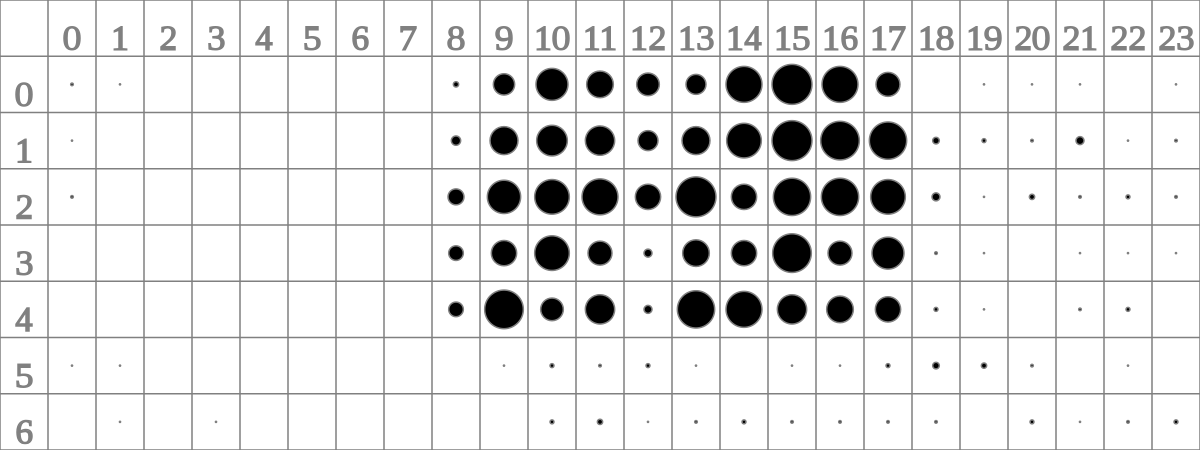
\includegraphics[width=0.9\textwidth]{img/punch_1.png}
        \\ \hfill \small Alan, Microblogging
      }

      \only<3>{
        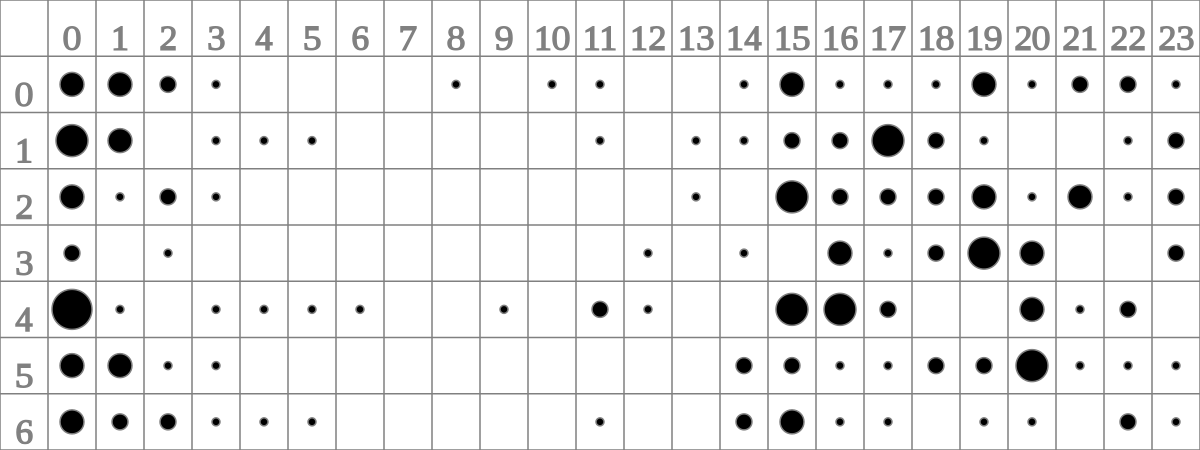
\includegraphics[width=0.9\textwidth]{img/punch_2.png}
        \\ \hfill \small Bob, Microblogging
      }

      \only<4>{
        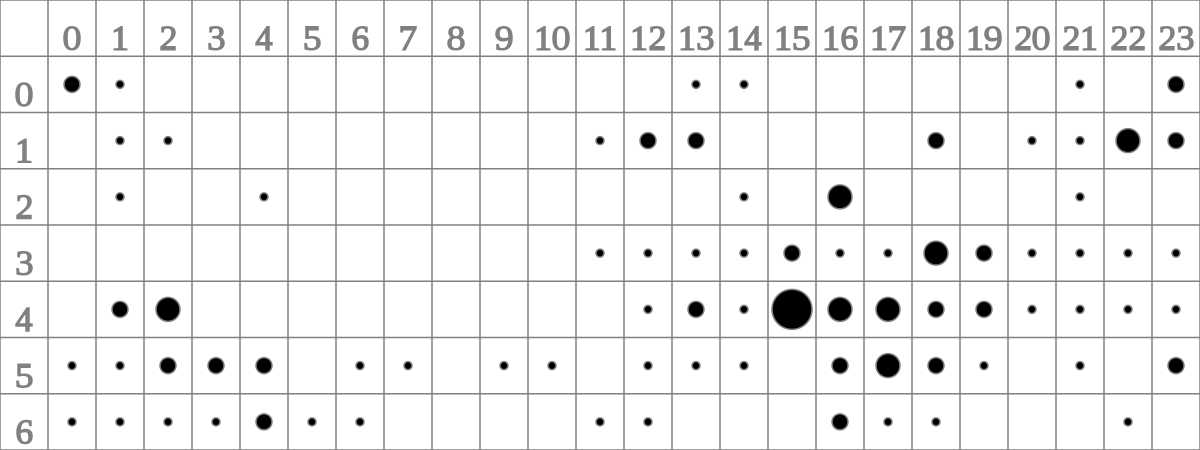
\includegraphics[width=0.9\textwidth]{img/punch_3.png}
        \\ \hfill \small Charlie, Github
      }
    \end{center}
\end{frame}

\begin{frame}
  \frametitle{Data Mining}
  \pause
  \begin{center}
    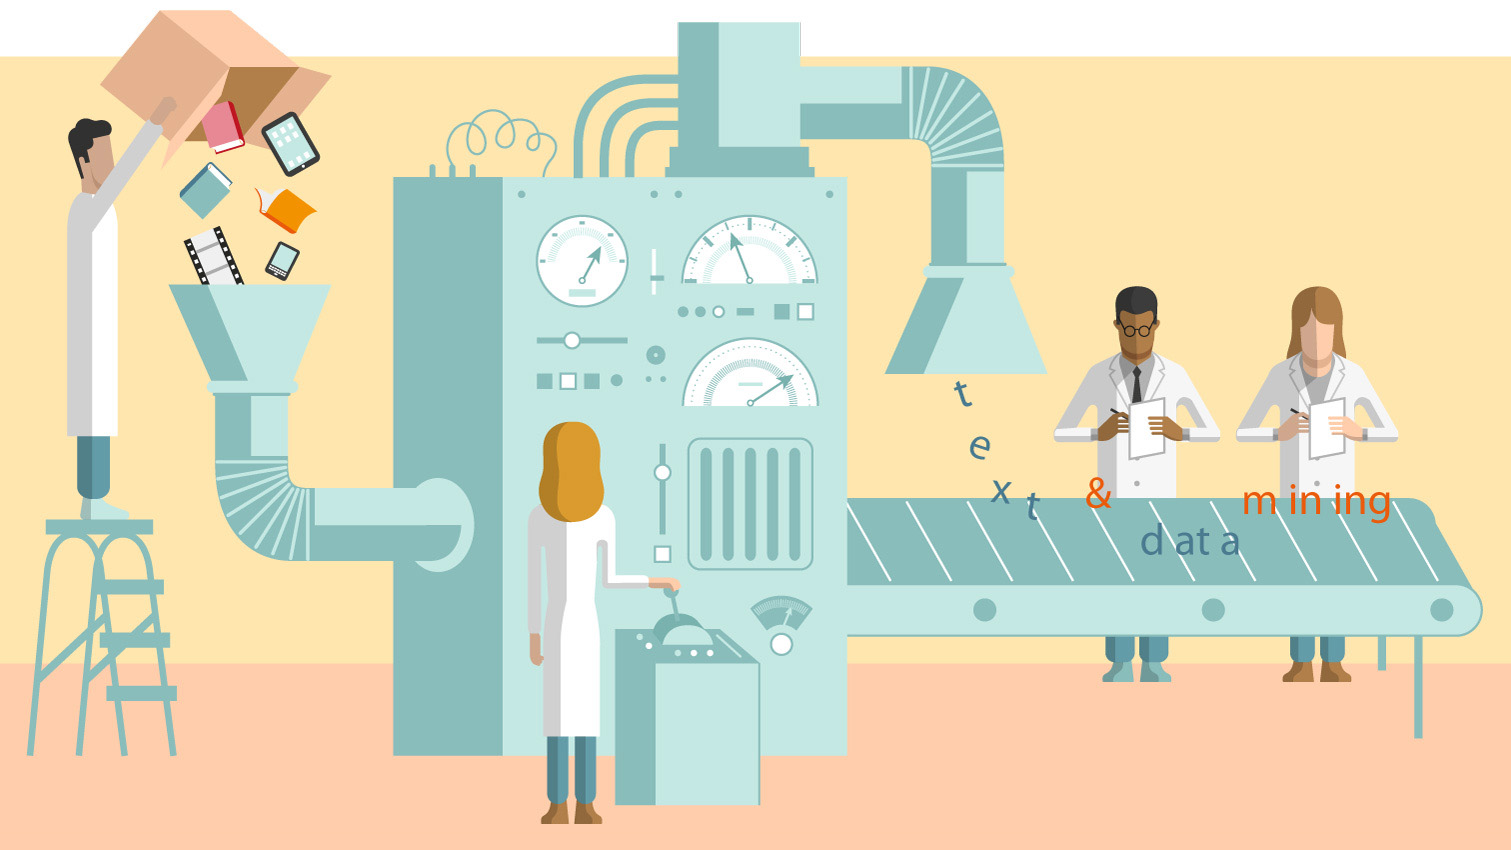
\includegraphics[width=0.8\textwidth]{img/text_data_mining.jpg}
    \license[http://copyrightuser.org/topics/text-and-data-mining/]{\cc{by}}
  \end{center}
\end{frame}

\end{document}

